\TieudeT{PHONG TỎA VẬT LÍ}
\subsubsection*{PHẦN I. Thí sinh trả lời câu hỏi từ câu 1 đến câu 18. Mỗi câu hỏi thí sinh chỉ chọn một phương án}
\setcounter{ex}{0}
%mac
\begin{ex}%Tailieuchuan
\immini[thm]{Một vật khối lượng $0,5 \ kg$ nằm trên mặt phẳng nghiêng góc $40^\circ$. Lấy $g=10 \ m/s^2$. Áp lực mà vật tác dụng lên mặt phẳng nghiêng có độ lớn là
\choice
{$6,83 \ N$}
{\True $3,83 \ N$}
{$5,12 \ N$}
{$8,31 \ N$}
}{
\includegraphics[width=4cm]{images/2025_04_24_746f9b43406b3514a111g-10}}
\loigiai{}
\end{ex}
\begin{ex}%Tailieuchuan
Một cần cẩu kéo một thùng containner khối lượng $5$ tấn từ trạng thái nghỉ lên độ cao $16\ m$ trong thời gian $4$ giây bằng một sợi dây cáp. Lấy $g=10 \ m/s^2$. Lực căng của dây cáp là
\choice
{\True $6.10^4\ N$}
{$4.10^4\ N$}
{$5.10^4\ N$}
{$8.10^4\ N$}
\loigiai{}
\end{ex}
\begin{ex}%Tailieuchuan
Một thùng gỗ đặt trên mặt phẳng nằm ngang được kéo bởi lực $F=10\ N$ theo phương hợp với phương ngang một góc $60^\circ$. Thùng chuyển động thẳng đều. Vật có khối lượng $5\ kg$. Lực ma sát có độ lớn là
\choice
{$1\ N$}
{$2\ N$}
{\True $5\ N$}
{$10\ N$}
\loigiai{}
\end{ex}
\begin{ex}%Tailieuchuan
\immini[thm]{Kéo vật nặng $2\ kg$ bằng lực $F=2 \ N$ làm vật chuyển động thẳng đều.  Lấy $g=10 \ m/s^2$. Hệ số ma sát trượt giữa vật và sàn là
\choice
{\True $0,1$}
{$0,2$}
{$0,25$}
{$0,15$}}{	
\includegraphics[width=4cm]{images/2025_04_24_2cebfca167c473dc9cdfg-20}
}
\loigiai{}
\end{ex}
\begin{ex}%Tailieuchuan
Cho một dốc con dài $50\ m$, cao $30\ m$. Cho một vật có khối lượng $m$ đang chuyển động thẳng đều với tốc độ $v_0$ trên mặt phẳng nằm ngang thì lên dốc. Biết hệ số ma sát giữa vật và dốc là $\mu=0,25$. Lấy $g=$ $10 \ m/s^2$. Tốc độ $v_0$ của vật trên mặt phẳng ngang để vật dừng lại ngay đỉnh dốc là
\choice
{\True $20 \sqrt{2} \ m/s$}
{$10 \sqrt{2} \ m/s$}
{$5 \sqrt{2} \ m/s$}
{$15 \sqrt{2} \ m/s$}
\loigiai{}
\end{ex}
\begin{ex}%Tailieuchuan
Một vật khối lượng $m$ trượt không vận tốc đầu từ đỉnh mặt phẳng nghiêng không ma sát. Biết góc nghiêng là $60^\circ$ và gia tốc trọng trường $g=10 \ m/s^2$. Gia tốc của vật khi di chuyển trên mặt phẳng nghiêng là
\choice
{$5 \ m/s^2$}
{$5 \sqrt{2} \ m/s^2$}
{\True $5 \sqrt{3} \ m/s^2$}
{$\dfrac{5}{\sqrt{2}} \ m/s^2$}
\loigiai{}
\end{ex}
\begin{ex}%book
Người ta đẩy một cái thùng có khối lượng $55\ kg$ theo phương ngang với lực $220\ N$ làm thùng chuyển động trên mặt phẳng ngang. Hệ số ma sát trượt giữa thùng và mặt phẳng là $0,35$. Lấy $g = 9,8\ m/s^2$. Gia tốc của thùng có độ lớn là
\choice
{\True $0,57\ m/s^2$}
{$1,57\ m/s^2$}
{$0,17\ m/s^2$}
{$3,67\ m/s^2$}
\haidong{6}\loigiai{
\immini{\begin{itemize}
\item Phương pháp giải:\\
Các bước giải bài toán phần động lực học:\\
Bước 1: Phân tích lực tác dụng lên vật	
Bước 2: Chọn hệ quy chiếu\\
Bước 3: Viết phương trình theo định luật 2 Newton: $\sum \vec F=m\vec a$\\
Bước 4: Chiếu phương trình định luật 2 Newton lên trục Ox và Oy $\Rightarrow$ Đại lượng cần tính
\item Vật chịu tác dụng của 4 lực: lực đẩy $\vec F$, lực ma sát $\vec F_{ms}$, trọng lực $\vec P$, phản lực $\vec N$. 
\item Chọn hệ quy chiếu và các lực có chiều như hình vẽ.
\item Theo định luật 2 Newton, ta có: $\vec F+\vec F_{ms}+\vec P+\vec N=m.\vec a$\quad (1)
\item Chiếu (1) lên trục Ox ta có: $F-F_{ms}=ma\Leftrightarrow F-\mu N=ma$\quad (2)
\item Chiếu (1) lên Oy, ta có: $P-N=0\Leftrightarrow N=P=mg$
\item Thay $N = mg$ vào (2), ta có: $F-\mu mg=ma\Leftrightarrow a=\dfrac{F-\mu mg}{m}=0,57\ m/s^2$.
\end{itemize}}{\begin{tikzpicture}[scale=1,thick,>=stealth']
\tkzDefPoints{0/1/o}
\node  at  (0,0.32)  [shape=rectangle,draw=red,pattern=dots,minimum height=0.6cm,minimum width=1.4cm, rounded corners=1pt]  {};
\draw(-1.5,0)--(1.5,0);
\draw[very thick,blue,->](0.1,0)--++(90:1.8)node[right,black]{$\vec{N}$};
\draw[fill=white](0.1,0)circle(1.2pt);
\draw[very thick,blue,->](0,0.32)--++(-90:1.8)node[right,black]{$\vec{P}$};
\draw[fill=white](0,0.32)circle(1.2pt);
\draw[very thick,blue,->](-0.7,0)--++(180:1.2)node[above,black]{$\vec{F}_{ms}$};
\draw[fill=white](-0.7,0)circle(1.2pt);
\draw[very thick,blue,->](0.7,0.32)--++(0:2)node[above,black]{$\vec{F}$};
\draw[fill=white](0.7,0.32)circle(1.2pt);
\fill[pattern=north east lines](-1.5,0)--(1.5,0)--++(-90:0.1)--++(180:3);
\draw[->](2,1)node[below left]{$O$}--++(90:1.5)node[right]{$y$};
\draw[->](2,1)--++(0:2)node[above]{$x$};
\end{tikzpicture}}
}	
\end{ex}
\begin{ex}%book
Một vật có khối lượng $2\ kg$ đặt nằm yên trên mặt bàn nằm ngang. Hệ số ma sát trượt giữa vật và mặt bàn là 0,5. Tác dụng lên vật một lực có độ lớn là $14\ N$, có phương song song với mặt bàn. Cho $g=10\ m/s^2$. Độ lớn gia tốc của vật bằng
\choice
{$3\ m/s^2$}
{$1,5\ m/s^2$}
{$5\ m/s^2$}
{\True $2\ m/s^2$}
\haidong{6}\loigiai{

Chọn D
\begin{itemize}
\item Vật chỉ chuyển động theo phương ngang nên $P$ và $Q$ cân bằng nhau.
\end{itemize}

\begin{center}
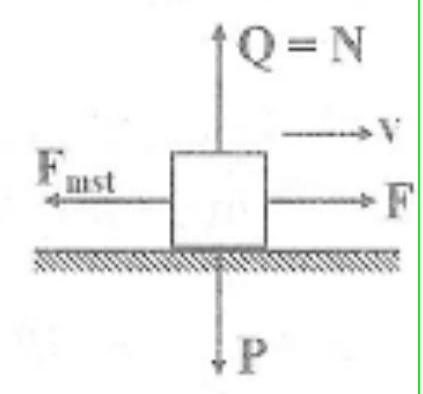
\includegraphics[width=4cm]{Images/2023_11_30_708f45f48fb252b4634cg-09}
\end{center}

\begin{itemize}
\item Chọn chiều dương là chiều chuyển động của vật.
\item Theo định luật II Niu-tơn:
\end{itemize}

$
a=\dfrac{F-\dot{F}_{m s}}{m}=\dfrac{F-\mu m g}{m}=\dfrac{14-0,5 .  2 .  10}{2}=2\ m/s^2
$

}
\end{ex}
\begin{ex}%book
Một ôtô có khối lượng $1$ tấn đang chuyển động với v $=54\ km/h$ thì tắt máy, hãm phanh, chuyển động chậm dần đều. Biết độ lớn lực hãm $3000\ N$. Quãng đường xe đi được cho đến khi dừng lại là
\choice
{$486\ m$}
{$0,486\ m$}
{\True $37,5\ m$}
{$18,75\ m$}
\haidong{6}\loigiai{

Chọn C
Chọn chiều + là chiều chuyển động, gốc thời gian lúc bắt đầu hãm phanh.

$
\begin{aligned}
& a=\dfrac{F}{m}=\dfrac{-3000}{1000}=-3\ m/s^2 \\
& v^2-v_0^2=2 .  a. s \Rightarrow s=37,5\ m
\end{aligned}
$

}
\end{ex}

\begin{ex}%book
Một máy bay trực thăng đang nâng một vật khối lượng $1500\ kg$ bằng một sợi dây. Lấy $g=9,8\ m/s^2$. Máy bay trực thăng và vật đang tăng tốc hướng lên với gia tốc $1 \ m/s^2$. Lực căng của sợi dây có độ lớn là
\choice
{$12,7.10^3\ N$}
{\True $16,2.10^3\ N$}
{$24,3.10^3\ N$}
{$18,8.10^3\ N$}
\haidong{6}\loigiai{
Chọn B
Các lực tác dụng vào khối vật: Trọng lực $\vec{P}$, lực căng dây $\vec{T}$

\begin{center}
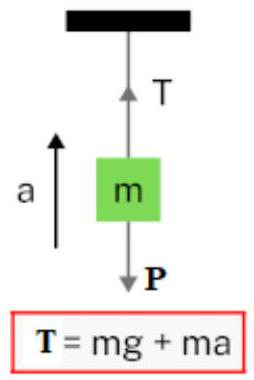
\includegraphics[width=4cm]{Images/2023_11_19_4b5f28cc74af8d9f8b65g-15}
\end{center}

Áp dụng định luật II Niwton: $\overrightarrow{P}+\overrightarrow{T}=ma$

Chiếu theo chiều của lực căng $\vec{T}$ ta được:

-Vật chuyển động đi lên với gia tốc a: $T-P=m a \Rightarrow T=m g+m a=16,2 .  10^3 \ N$

}
\end{ex}
\begin{ex}%book
Một cần cẩu được sử dụng để nâng một vật có khối lượng $500\ kg$ với gia tốc $1\ m/s^2$ theo phương thẳng đứng. Lấy $g=9,8\ m/s^2$. Lực căng dây cáp giữa cầu trục và vật có độ lớn là
\choice
{$6700 \ N$}
{$500 \ N$}
{\True $5400 \ N$}
{$3500 \ N$}
\haidong{6}\loigiai{
Các lực tác dụng vào khối vật: Trọng lực $\vec{P}$, lực căng dây $\vec{T}$

\begin{center}
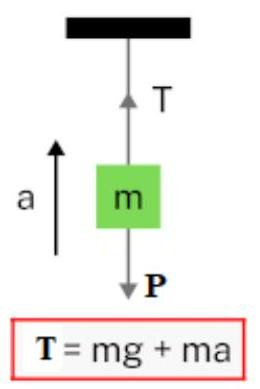
\includegraphics[width=4cm]{Images/2023_11_19_4b5f28cc74af8d9f8b65g-15(1)}
\end{center}

Áp dụng định luật II Niwton: $\vec{P}+\vec{T}=m \vec{a}$

Chiếu theo chiều của lực căng $\vec{T}$ ta được:

-Vật chuyển động đi lên với gia tốc a: $T-P=m a \Rightarrow T=m g+m a=5400 \ N$

}
\end{ex}

\begin{ex}%book
\immini[thm]{Cho một vật có khối lượng $100\ kg$ đặt trên mặt phẳng nằm ngang. Kéo vật bằng lực $\vec{F}$ hợp với phương ngang một góc $\alpha=30^\circ$ để vật chuyển động đều. Biết hệ số ma sát giữa vật và mặt phẳng là $\mu=0,2$. Lấy $g=10\ m/s^2$. Độ lớn của lực $F$ là
\choice
{$240\ N$}
{\True $207\ N$}
{$150\ N$}
{$187\ N$}}{
\begin{tikzpicture}[scale=1,thick,>=stealth']
\node  at  (0,0.32)  [shape=rectangle,draw=red,pattern=dots,minimum height=0.6cm,minimum width=1.4cm, rounded corners=1pt]  {};
\draw(-1.5,0)--(1.5,0);
\draw[very thick,blue,->](0.7,0.3)--++(30:2)node[right,black]{$\vec{F}$}coordinate(f);
\draw[fill=white](0.7,0.3)circle(1.2pt);
\draw[dashed](0.7,0.3)coordinate(o)--(2.3,0.3)coordinate(fx);
\tkzMarkAngles[size=0.7cm](fx,o,f)
\tkzLabelAngles[pos=1](fx,o,f){$\alpha$}
\fill[pattern=north east lines](-1.5,0)--(1.5,0)--++(-90:0.1)--++(180:3);
\end{tikzpicture}}

\haidong{10}	\loigiai{

Chọn B

$+F \cos \alpha=\mu(m g-F \sin \alpha) \Rightarrow F=\dfrac{\mu m g}{\cos \alpha+\mu \sin \alpha}=207 N$


}
\end{ex}




\begin{ex}%book
Một học sinh dùng dây kéo một thùng sách nặng 10 kg chuyển động trên mặt sàn nằm ngang. Dây nghiêng một góc chếch lên trên $30^\circ$ so với phương ngang. Hệ số ma sát trượt giữa đáy thùng và mặt sàn là $\mu =0,2$. Lấy $g=9,8\ m/s^2$. Độ lớn của lực kéo để thùng sách chuyển động thẳng đều là
\choice
{\True $20,3\ N$}
{$32,0\ N$}
{$30,2\ N$}
{$32,2\ N$}
\haidong{10}\loigiai{
\begin{itemize}
\item $\vec F+\vec P+\vec N+\vec F_{ms}=\vec 0$
\item Thay số: $F=20,3\ N$,
\end{itemize}	
}
\end{ex}
\begin{ex}%Tailieuchuan
Một cần cẩu kéo một cái tủ gỗ khối lượng $500\ kg$ lên cao. Biết rằng trên nửa quãng đường đầu tủ được kéo lên thẳng nhanh dần đều với gia tốc a và trên nửa quãng đường sau tủ được kéo lên thẳng chậm dần đều với gia tốc có cùng độ lớn. Biết lực căng dây trên nửa quãng đường đầu gấp $1,5$ lần lực căng dây trên nửa quãng đường sau. Lấy $g=10 \ m/s^2$. Bỏ qua khối lượng dây nối. Gia tốc trên nửa quãng đường đầu là
\choice
{\True $2 \ m/s^2$}
{$4 \ m/s^2$}
{$0,5 \ m/s^2$}
{$1 \ m/s^2$}
\loigiai{}
\end{ex}


















\textit{Sử dụng thông tin sau cho Câu 15 và Câu 16:} Hai vật có khối lượng lần lượt là $m_1=5\ kg$ và $m_2=10\ kg$ được nối với nhau bằng một sợi dây không dãn và được đặt trên một mặt sàn nằm ngang. Kéo vật $1$ bằng một lực $\vec F$ nằm ngang không ma sát có độ lớn $F=12\ N$.
\begin{ex}%book
 Gia tốc của mỗi vật có độ lớn là
\choice
{\True $0,8\ m/s^2$}
{$1\ m/s^2$}
{$1,2\ m/s^2$}
{$2,4\ m/s^2$}
\haidong{10}\loigiai{
\begin{itemize}
\item $a=\dfrac{F}{m_1+m_2}=0,8\ m/s^2$.
\end{itemize}	
}
\end{ex}
\begin{ex}%book
 Lực căng của dây nối có độ lớn là
\choice
{\True $8\ N$}
{$10\ N$}
{$12\ N$}
{$24\ N$}
\haidong{10}\loigiai{
\begin{itemize}
\item $T=m_2a=8\ N$.
\end{itemize}	
}
\end{ex}
\textit{Sử dụng thông tin sau cho Câu 15 và Câu 16:} Hai vật có khối lượng lần lượt là $m_1=5\ kg$ và $m_2=10\ kg$ được nối với nhau bằng một sợi dây không dãn và được đặt trên một mặt sàn nằm ngang. Kéo vật $1$ bằng một lực $F$ nằm ngang có độ lớn $F=45\ N$. Hệ số ma sát giữa mỗi vật và mặt sàn là $\mu=0,2$. Lấy $g=9,8\ m/s^2$. 	\haidong{15}
\begin{ex}
Gia tốc của mỗi vật có độ lớn là
\choice
{\True $1,04\ m/s^2$}
{$2,64\ m/s^2$}
{$3,65\ m/s^2$}
{$4,24\ m/s^2$}
\loigiai{
Cách 1:
\begin{center}
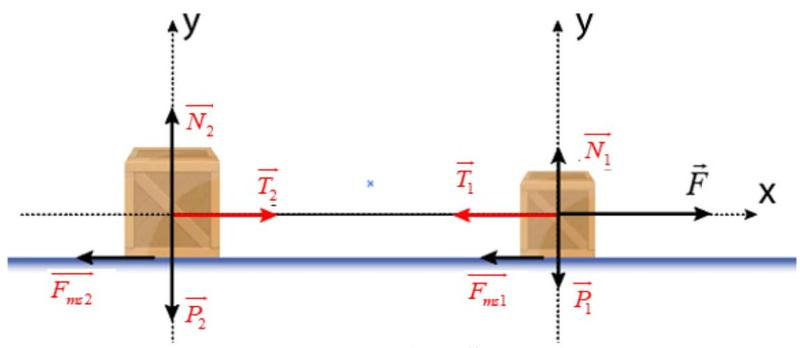
\includegraphics[width=10cm]{Images/2023_11_30_708f45f48fb252b4634cg-07}
\end{center}

Các lực tác dụng lên vật được biểu diễn như hình vẽ.

Xét vật 2:
Coi vật 1 như một chất điểm:

Áp dụng định luật II Newton theo các trục $O x$ và $O y$:

Oy: $N_2=P_2=m_2 g$

Mà $F_{m s 2}=\mu. N_2=\mu. m_2 g$

$O x: T_2-F_{m s 2}=m a_2 \Rightarrow T_2-\mu .  m_2 g=m_2 .  a_2 \Rightarrow T_2=\mu .  m_2 g+m_2 .  a_2$

Xét vật 1:
Oy: $N_1=P_1=m_1 g \Rightarrow F_{m s 1}=\mu N_1=\mu m_1 g$

OX: Tương tự, ta có: $F-T_1-F_{m s 1}=m a_1 \Rightarrow T_1=F-\mu m_1 g-m_1 a_1$

Mà sợi dây nhẹ, không dãn nên $T=T_1=T_2$ và $a_1=a_2$.

Suy ra: $\mu .  m_2 g+m_2 .  a=F-\mu m_1 g-m_1 a$

$\Rightarrow a\left(m_1+m_2\right)=F-\mu g\left(m_2+m_1\right)$

$a=\dfrac{F}{m_1+m_2}-\mu g=\dfrac{45}{5+10}-0,2.9.8=1,04\ m/s^2$

Cách 2:
\begin{center}
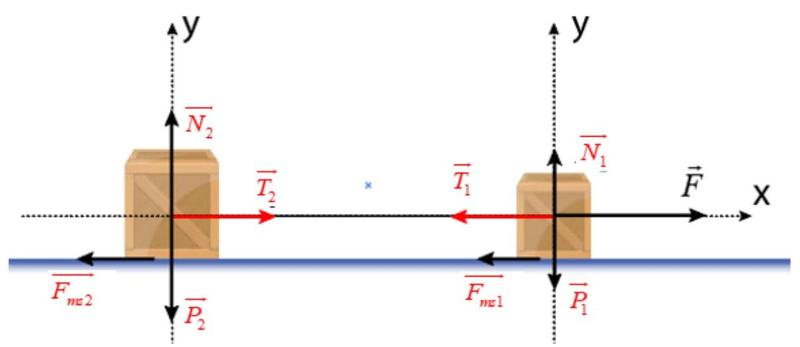
\includegraphics[width=10cm]{Images/2023_11_30_708f45f48fb252b4634cg-08(1)}
\end{center}

Xét 2 vật là một hệ tổng thể.

Áp dụng định luật II Newton cho hệ vật: $\vec{F}+\vec{F}_{m s 1}+\vec{P}_1+\vec{N}_1+\vec{F}_{m s 2}+\vec{P}_2+\vec{N}_2=\left(m_1+m_2\right) \vec{a}(1)$

\begin{itemize}
\item Chọn hệ Oxy như hình vẽ.
\end{itemize}

Chiếu (1)/Oy, ta có: $N_1+N_2=P_1+P_2=g . \left(m_1+m_2\right)$

Chiếu (1)/Ox, ta có

$
\begin{aligned}
& F-F_{m s_1}-F_{m s_2}=\left(m_1+m_2\right) a \\
& \Rightarrow a=\dfrac{F-\mu N_1-\mu N_2}{m_1+m_2} \\
& =\dfrac{F-\mu g\left(m_1+m_2\right)}{m_1+m_2} \\
& =\dfrac{F}{m_1+m_2}-\mu g \\
& =\dfrac{45}{5+10}-0,2.9.8=1,04\ m/s^2
\end{aligned}
$
}
\end{ex}
\begin{ex}
Lực căng của dây nối có độ lớn là
\choice
{\True $30\ N$}
{$40\ N$}
{$50\ N$}
{$60\ N$}
\loigiai{
Cách 1:

$T=T_1=T_2=\mu .  m_2 g+m_2 .  a=m_2(\mu .  g+a)=10 . (0,2.9,8+1,04)=30\ N$

Cách 2:

$T-F_{m s 2}=m_2 a=>T=F_{m s 2}+m_2 a=\mu .  m_2 g+m_2 .  a=m_2(\mu .  g+a)=10 . (0,2 .  9,8+1,04)=30 N$

}
\end{ex}



\subsubsection*{PHẦN 2. Thí sinh trả lời từ câu 1 đến câu 4. Trong mỗi ý a), b), c), d) ở mỗi câu, thí sinh chọn đúng hoặc sai.}
\setcounter{ex}{0}
\begin{ex}%Tailieuchuan
\immini[thm]{Một vật khối lượng $m=2 \ kg$ nằm cân bằng trên một mặt phẳng nghiêng nhờ một sợi dây song song với mặt phẳng nghiêng như hình vẽ. Góc nghiêng $\alpha=30^\circ$. Bỏ qua ma sát giữa vật và mặt phẳng nghiêng. Lấy $g=10 \ m/s^2$.}{
\begin{tikzpicture}[scale=0.8,thick,>=stealth',draw=Mapcolor]
\tkzInit[ymin=-3.5,ymax=0.2,xmin=-0.5,xmax=5.5]\tkzClip
\begin{scope}[shift={(0,0)},rotate=-30]
\node  at  (3.3,0)  [shape=rectangle,draw=red,pattern=dots,minimum height=0.45cm,minimum width=0.6cm, rounded corners=1pt,rotate=-30]  {};
\draw(0,0) -- (3,0);
\draw(0,0.27)--(0,-0.27)coordinate(a)--++(0:6)coordinate(b)--++(210:5)coordinate(c);
\fill[pattern=horizontal lines](0,0.27)--(0,-0.27)--++(180:0.1)--++(90:0.54);
\fill[pattern=north east lines](b)--(c)--++(300:0.1)--++(390:5);
\tkzMarkAngles[size=0.5cm](a,b,c)
\tkzLabelAngle[pos=-0.8](a,b,c){$\alpha$}
\end{scope}
\end{tikzpicture}}
\choiceTF[t]
{\True Vật nằm cân bằng nên hợp lực tác dụng lên vật bằng $0\ N$} 
{Các lực tác dụng lên vật gồm: trọng lực, phản lực, lực căng dây và lực ma sát} 
{\True Lực căng của dây là $10\ N$} 
{Phản lực do mặt nghiêng tác dụng lên vật có độ lớn $20\ N$} 
\loigiai{
}
\end{ex}
\begin{ex}%Tailieuchuan
\immini[thm]{Hình dưới biểu diễn quả tennis đang rơi thẳng đứng trong không khí. Trong quá trình rơi, quả tennis chỉ chịu tác dụng bởi hai lực như hình vẽ. Biết khối lượng quả tennis là $56\ g$. Biết lực $\vec{D}$ có độ lớn là $0,2 \ N$ và gia tốc trọng trường $g=9,8 \ m/s^2$.}{

\includegraphics[width=2cm]{images/2025_04_24_509886e0d712477af59ag-11(1)}}
\choiceTF[t]
{\True Lực $\vec{D}$ cản trở chuyển động của quả tennis} 
{\True Lực $\vec{D}$ có độ lớn nhỏ hơn trọng lực} 
{Chuyển động của quả tennis là chuyển động rơi tự do} 
{\True Gia tốc của quả tennis khoảng $6,23 \ m/s^2$} 
\loigiai{ 
\begin{itemchoice}
\itemch
\itemch
\itemch
\itemch
\end{itemchoice}
}
\end{ex}

\begin{ex}%book
Một ô tô đang chuyển động với vận tốc không đổi $30\ m / s$. Đến chân một con dốc, đột nhiên tắt máy ngừng hoạt động và ô tô theo đà đi lên dốc. Nó luôn luôn chịu một gia tốc ngược chiều với vận tốc ban đầu và gia tốc có độ lớn $2\ m / s^{2}$ trong suốt quá trình lên dốc và xuống dốc. Lấy gốc tọa độ $x=0$ tại chân dốc, chiều dương là chiều lên dốc và gốc thời gian $t=0$ là lúc xe ở vị trí chân dốc. 
\choiceTF[t]
{Quãng đường xa nhất trên sườn dốc mà xe có thể lên được là $220\ m$}
{\True Thời gian để xe đi hết quãng đường này là $15\ s$}
{Sau 20 s , vận tốc của ô tô là $10 \ m/s$}
{\True Tại thời điểm $t=20~s$, ô tô chuyển động ngược chiều dương (xuống dốc)}

\loigiai{\begin{itemchoice}
\itemch Sai. Ta có: $v^{2}-v_{0}^{2}=2 a S \Rightarrow S=\dfrac{v^{2}-v_{0}^{2}}{2 a}=\dfrac{0^{2}-30^{2}}{2 .(-2)}=225(~m)$.
\itemch Đúng. Thời gian để xe đi hết quãng đường này là $t=\dfrac{v-v_{0}}{a}=\dfrac{-30}{-2}=15(~s)$
\itemch Sai. Sau 20 s , vận tốc của ô tô là $v=v_{0}+a t=30+(-2) . 20=-10\ m / s$
\itemch Đúng. Vì $v=v_{0}+a t=30+(-2) . 20=-10\ m / s<0$ nên ô tô đang chuyển động ngược chiều dương.
\end{itemchoice}
}

\end{ex}


\begin{ex}%book
Một vật trượt từ trạng thái nghỉ xuống một mặt phẳng nghiêng với góc nghiêng $30^{\circ}$ so với phương ngang. Biết hệ số ma sát trượt giữa vật và mặt phẳng nghiêng là $\dfrac{\sqrt{3}}{6}$. Lấy $g=9,8\ m / s^{2}$.
\choiceTF[t]
{\True Vật trượt nhanh dần đều}
{Khi không có ma sát, gia tốc của vật bằng gia tốc trọng trường}
{Khi có ma sát, gia tốc của vật là $4,9\ m /{s}^2$}
{Khi này, vật trượt được quãng đường $2,45 {~m}$ trong giây đầu tiên}

\loigiai{\immini{\begin{itemchoice}
\itemch Đúng.
\itemch Sai. Phương trình động lực học: $\vec{P}+\vec{N}+\vec{F}_{m s}=m \vec{a}$

Chiếu lên trục $O x$, ta có: $m a=P \sin \alpha-F_{m s}$

Chiếu lên trục $O y$, ta có: $0=N-P \cos \alpha$

$\Rightarrow N=P \cos \alpha=m g \cos \alpha \Rightarrow F_{m s}=\mu N=\mu m g \cos \alpha$

Nếu bỏ qua ma sát, ta có: $a=g . \sin \alpha$.

\itemch Sai. Trường hợp có ma sát

$a=g(\sin \alpha-\mu . \cos \alpha)=9,8 .\left(\sin 30^{\circ}-\dfrac{\sqrt{3}}{6} . \cos 30^{\circ}\right)=2,45\ m / s^{2}$.

\itemch Sai. Quãng đường vật trượt được trong giây đầu tiên: $S=\dfrac{1}{2} a . t^{2}=\dfrac{1}{2} . 2,45 . 1^{2}=1,225\ m$.

\end{itemchoice}}{\begin{tikzpicture}[scale=1,thick,>=stealth']
\tkzInit[ymin=-4,ymax=1,xmin=-0.5,xmax=5.5]\tkzClip
\begin{scope}[shift={(0,0)},rotate=-30]
\node  at  (3.3,0)  [shape=rectangle,draw=red,pattern=dots,minimum height=0.5cm,minimum width=0.6cm, rounded corners=1pt,rotate=-30]  {};
\draw[very thick,blue,->](3,-0.25)coordinate(o)--++(180:0.7)node[below,black,xshift=-10pt]{$\vec{F}_{ms}$};
\draw[fill=white](3,-0.25)circle(1.2pt);
\draw[very thick,blue,->](3.3,0)--++(0:0.7)node[above,black,xshift=10pt]{$\vec{P}_x$}coordinate(px);
\draw[very thick,blue,->](3.3,0)coordinate(o')--++(90:1.2)node[right,black]{$\vec{N}$};
\draw[very thick,blue,->](3.3,0)--++(-90:1.2)node[left,black]{$\vec{P}_y$}coordinate(n);
\draw[very thick,blue,->](3.3,0)--++(-60:1.4)node[right,black,yshift=5pt]{$\vec{P}$}coordinate(p);
\draw[dashed,thin](px)--(p)--(n);
\draw[->](o)--++(0:2)node[above right,black]{$x$};
\draw[fill=white](3.3,0)circle(1.2pt);
\draw(0,-0.27)coordinate(a)--++(0:6)coordinate(b)--++(210:5)coordinate(c);
\fill[pattern=north east lines](b)--(c)--++(300:0.1)--++(390:5);
\tkzMarkAngles[size=0.5cm](a,b,c)
\tkzLabelAngle[pos=-0.8](a,b,c){$\alpha$}
\tkzMarkAngles[size=0.5cm](px,p,o')
\tkzLabelAngle[pos=0.7](px,p,o'){$\alpha$}
\end{scope}
\end{tikzpicture}}	
}
\end{ex}






















\subsubsection*{PHẦN 3. Thí sinh trả lời từ câu 1 đến câu 6.}
\setcounter{ex}{0} 
\begin{ex}%book
Khối gỗ khối lượng $20 \ kg$ đang được một sợi dây kéo thẳng đứng nhanh dần đều lên trên với gia tốc $25 \ m/s^2$. Lấy $g=9,8\ m/s^2$. Lực căng dây tác dụng lên khối gỗ có độ lớn là bao nhiêu niutơn?
\shortans[oly]{696}
\haidong{6}\loigiai{
\begin{center}
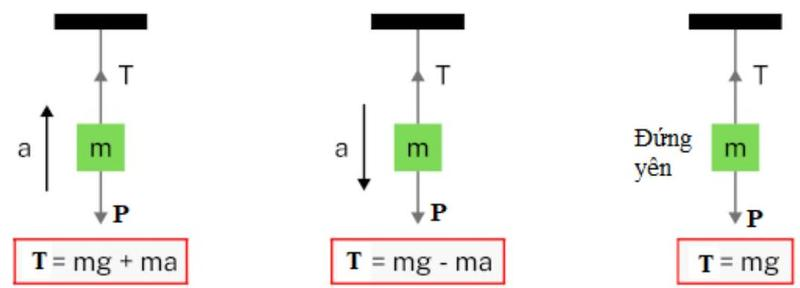
\includegraphics[width=12cm]{Images/2023_11_19_4b5f28cc74af8d9f8b65g-04(2)}
\end{center}

Các lực tác dụng vào khối vật: Trọng lực $\vec{P}$, lực căng dây $\vec{T}$

Áp dụng định luật II Niwton: $\vec{P}+\vec{T}=m \vec{a}$

Chiếu theo chiều của lực căng $\vec{T}$ ta được:
Vật chuyển động đi lên với gia tốc a: $T-P=m a \Rightarrow T=m g+m a=m(g+a)=20(10+25)=700 \ N$}
\end{ex}
\begin{ex}%book
Một học sinh dùng dây kéo một thùng sách nặng $10\ kg$ chuyển động trên mặt sàn nằm ngang. Dây nghiêng một góc chếch lên trên $45^\circ$ so với phương ngang. Hệ số ma sát trượt giữa dây thùng và mặt sàn là $\mu=0,2$. Lấy $g=9,8\ m/s^2$. Độ lớn của lực kéo để thùng sách chuyển động thẳng đều là bao nhiêu niutơn (làm tròn kết quả đến chữ số hàng phần mười)?
\shortans[oly]{23,1}
\haidong{10}
\loigiai{

Các lực tác dụng vào thùng sách khi nó trượt: Trọng lực $\vec{P}$; Lực ma sát trượt giữa vật và mặt sàn $\vec{F}_{m s}$; phản lực vuông góc với mặt sàn $\vec{N}$; lực kéo $\vec{F}$.

\begin{center}
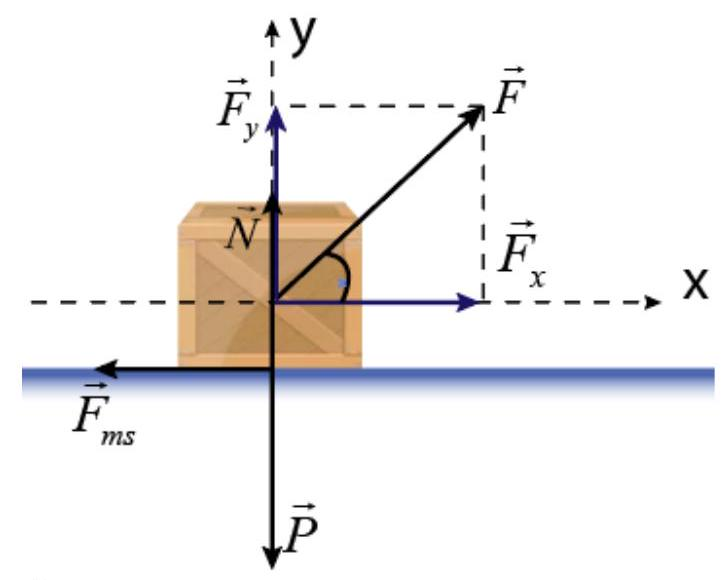
\includegraphics[width=6cm]{Images/2023_11_30_708f45f48fb252b4634cg-05(1)}
\end{center}

Áp dụng định luật II Newton theo các trục $O x$ và $O y$:

$O y: F_{y}+N-P=0 \Rightarrow F \sin 45^\circ+N-m g=0 \Rightarrow N=m g-F \sin 45^\circ$

mà $F_{m s}=\mu. N=\mu\left(m g-F \sin 45^\circ\right)$

$O x: F_{x}-F_{m s}=m a \Rightarrow F \cos 45^\circ-\mu\left(m g-F \sin 45^\circ\right)=m a \Rightarrow F \cos 45^\circ-\mu\left(m g-F \sin 45^\circ\right)=m a$

Thùng sách chuyển động đều nên $a=0$

$F \cos 45^\circ-\mu\left(m g-F \sin 45^\circ\right)=0$

$\Rightarrow F\left(\cos 45^\circ+\mu \sin 45^\circ\right)=\mu m g$

$\Rightarrow F=\dfrac{\mu m g}{\cos 45^\circ+\mu .  \sin 45^\circ}=\dfrac{0 .  2 .  10 .  9,8}{\cos 45^\circ+0,2 .  \sin 45^\circ} \approx 23,1 N$

}
\end{ex}
\begin{ex}%book
\immini[thm]{Một ô tô có khối lượng $1,2$ tấn đang lên dốc, biết dốc nghiêng $30^\circ$ so với mặt phẳng ngang. Lực phát động gây ra bởi động cơ ô tô có độ lớn $8000\ N$. Hệ số ma sát lăn giữa bánh xe và mặt đường là $\mu=0,05$. Cho $g=9,8\ m/s^2$. Gia tốc của xe khi lên dốc là bao nhiêu $m/s^2$ (làm tròn kết quả đến chữ số hàng phần trăm)?}{
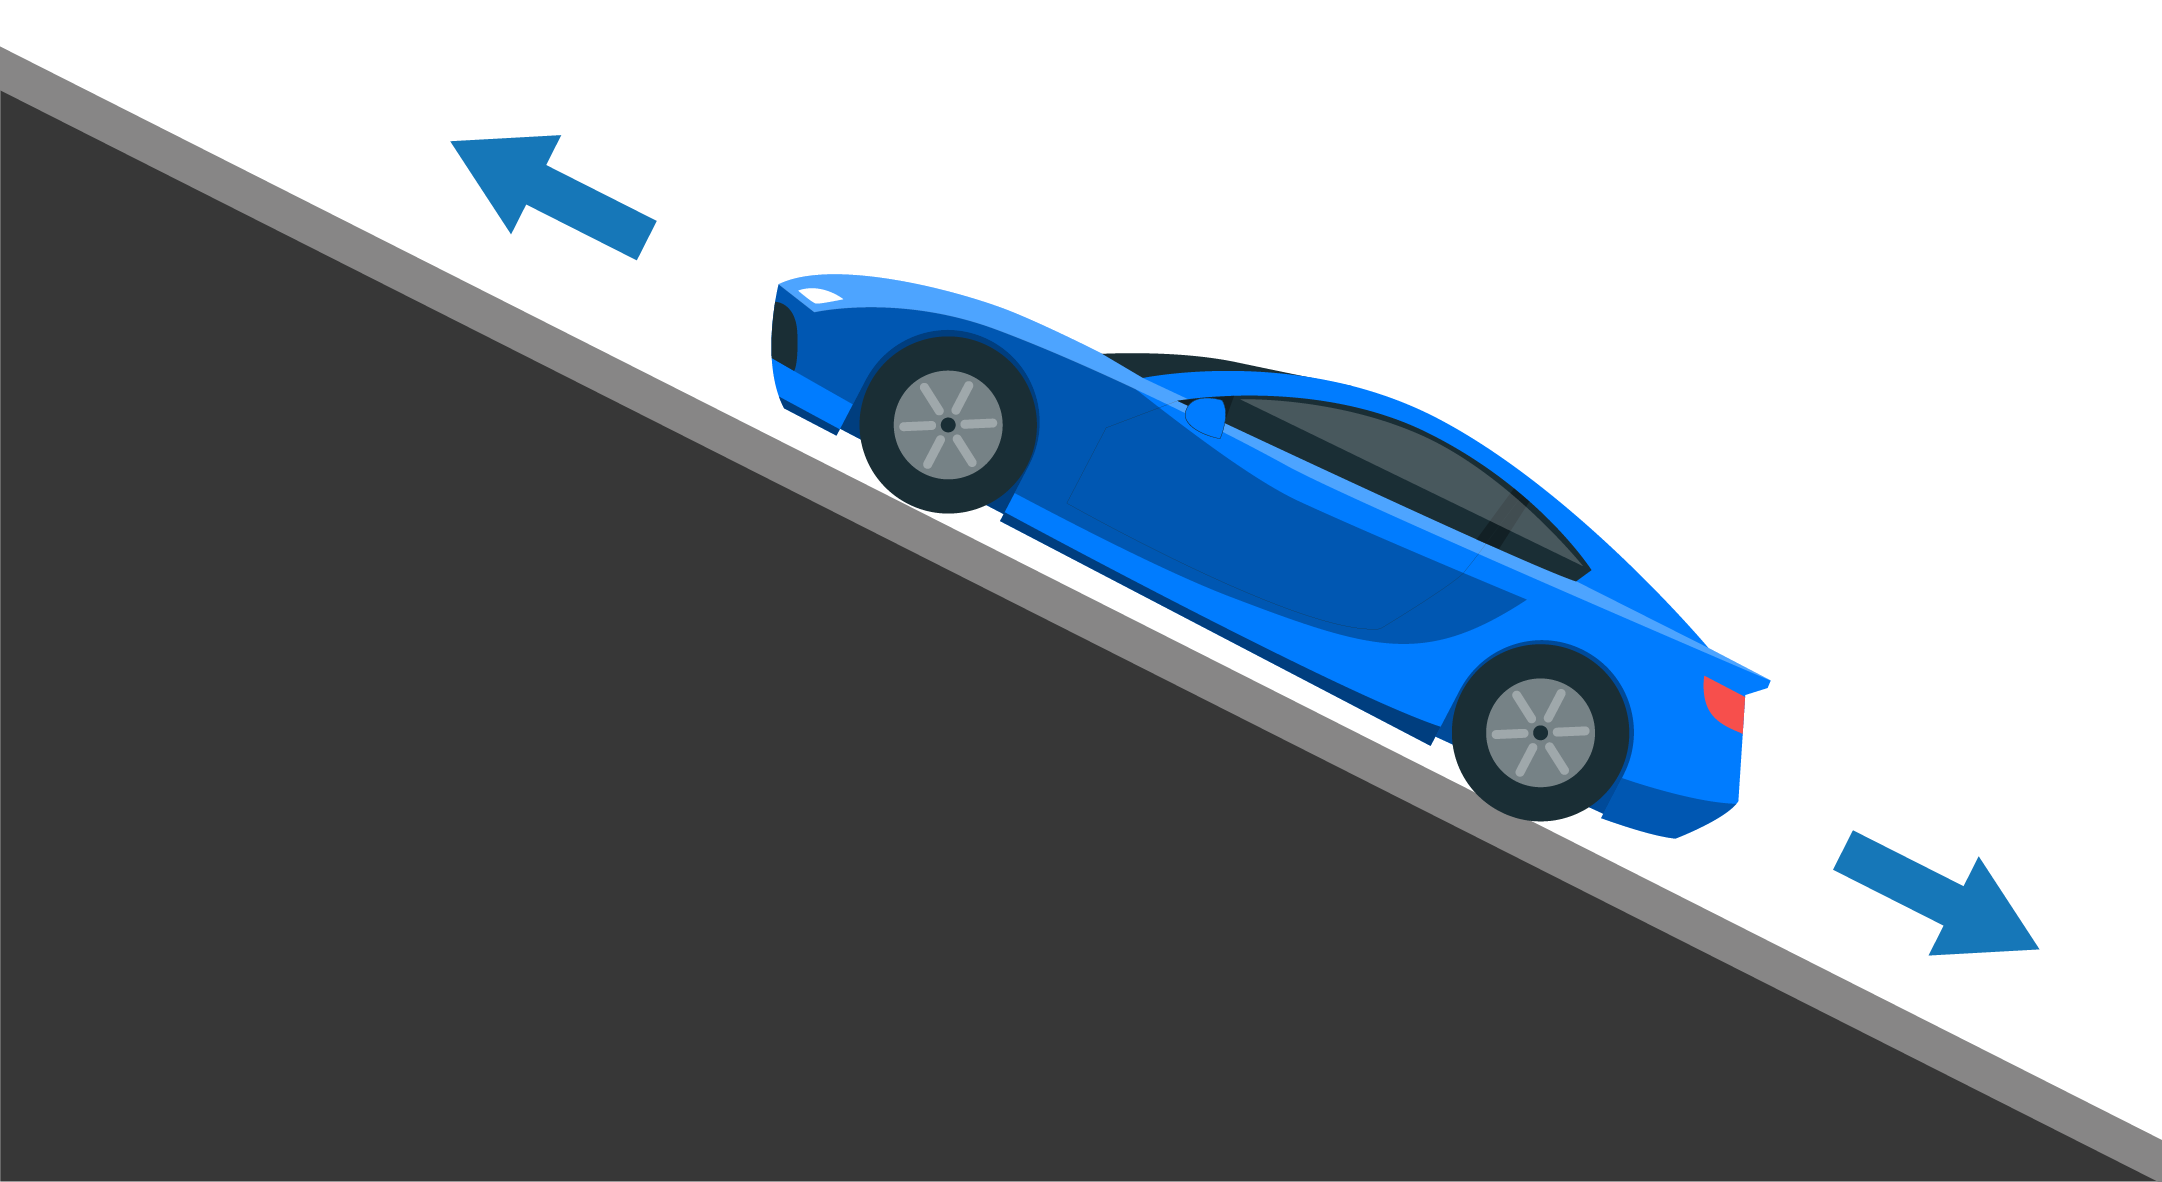
\includegraphics[width=4.75cm]{Images/89}}
\shortans[oly]{1,34}
\haidong{10}
\loigiai{

\begin{center}
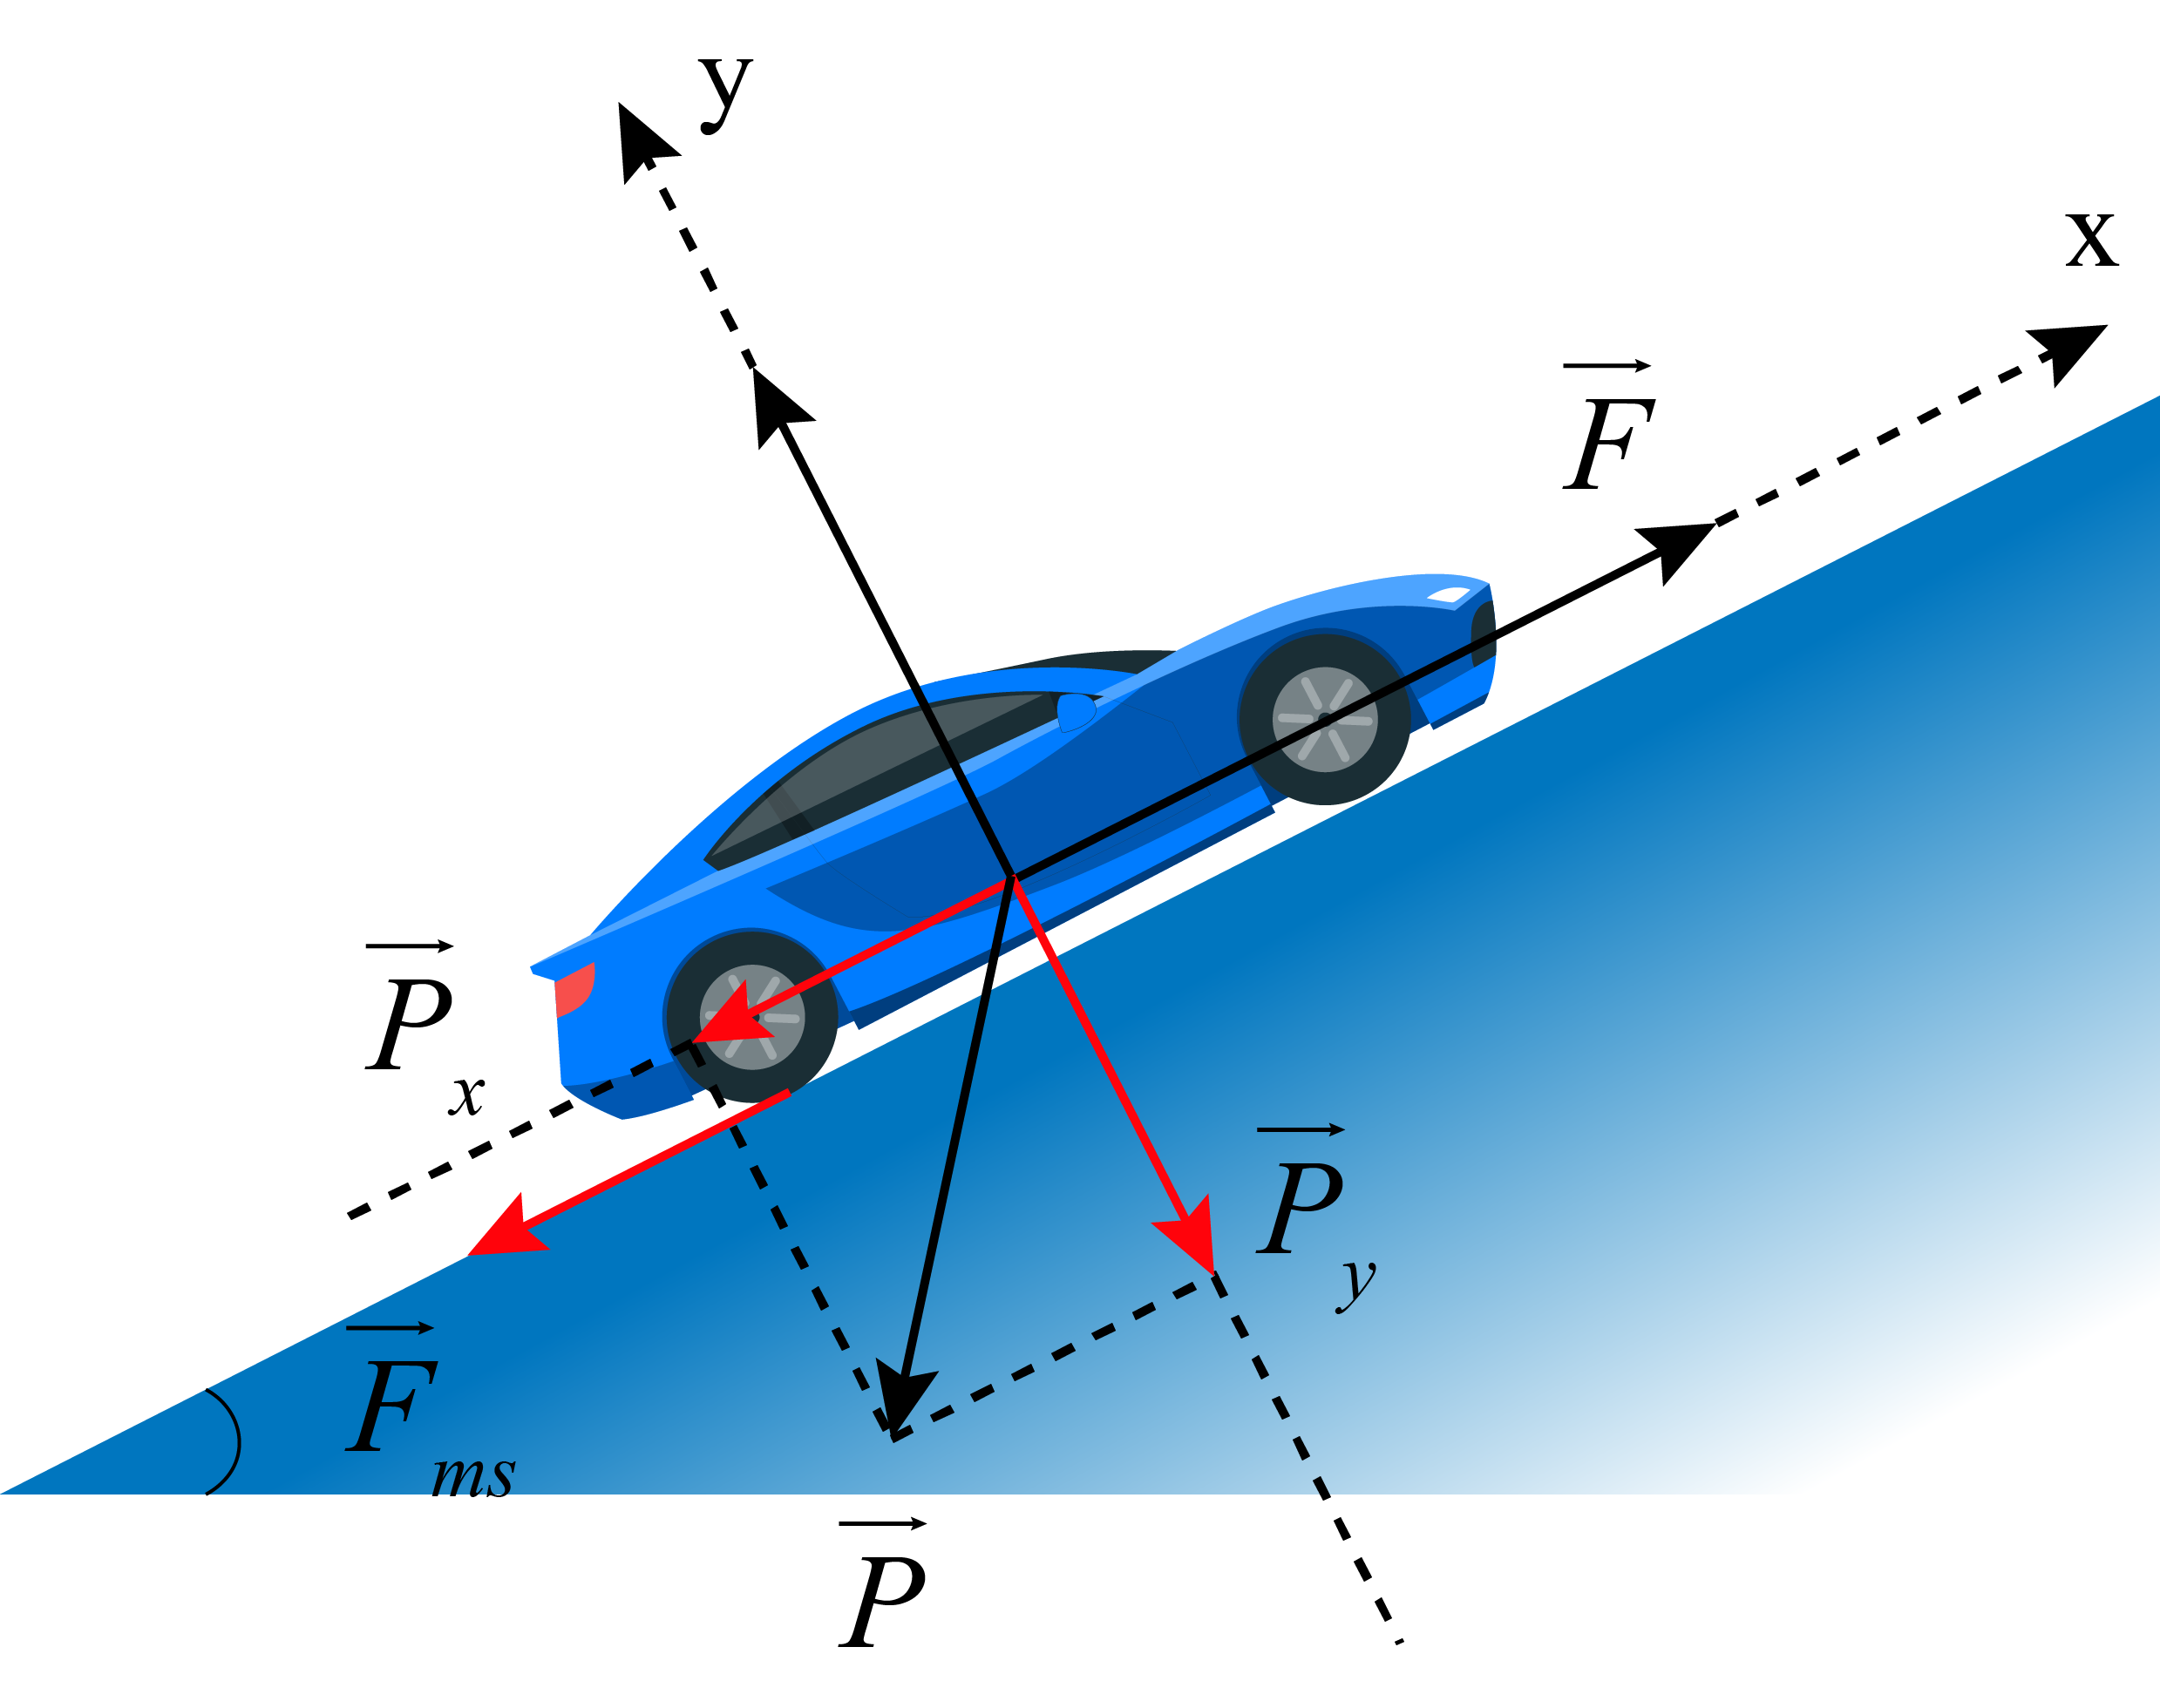
\includegraphics[width=8cm]{Images/2023_11_30_708f45f48fb252b4634cg-03(2)}
\end{center}

Các lực tác dụng vào xe khi lên dốc: Trọng lực $\vec{P}$; Lực ma sát trượt giữa xe và mặt đường $\vec{F}_{m s}$; phản lực vuông góc với mặt bàn $\vec{N}$; Lực phát động gây ra bởi động co ô tô có độ lớn $\vec{F}$.

Áp dụng định luật II Newton theo các trục $O x$ và $O y$:

Oy: $-P_{y}+N=0 \Rightarrow N=P_{y}=m g \cos \alpha$

Mà $F_{m s}=\mu .  N=\mu .  m g .  \cos \alpha$

$O x: F-F_{m s}-P_{x}=m a \Rightarrow F-\mu .  m g .  \cos \alpha-m g .  \sin \alpha=m a$

$\Rightarrow a=\dfrac{F}{m}-g . (\sin \alpha+\mu \cos \alpha)=\dfrac{8000}{1200}-9,8 . \left(\sin 30^\circ+0,05 .  \cos 30^\circ\right) \approx 1,34\ m/s^2$

}
\end{ex}
\begin{ex}%Tailieuchuan
Một chiếc xe ô tô có khối lượng tổng cộng người và xe là $550\ kg$ đang chuyển động trên mặt đường nằm ngang. Biết lực đẩy gây ra bởi động cơ tác dụng lên ô tô là $300\ N$ và tổng lực cản của môi trường lên ô tô là
$200\ N$. Gia tốc của ô tô có độ lớn là bao nhiêu $m/s^2$ (làm tròn kết quả đến chữ số hàng phần trăm)?
\shortans[oly]{0,18}
\loigiai{
}
\end{ex}




\textit{Sử dụng thông tin sau cho Câu 5 và Câu 6:} Một quyển sách đặt trên mặt bàn nghiêng và được thả cho trượt xuống. Cho biết góc nghiêng $\alpha=30^\circ$ so với phương ngang và hệ số ma sát giữa quyển sách và mặt bàn là $\mu =0,3$. Lấy $g = 9,8\ m/s^2$. 
\begin{ex}
Gia tốc của vật là bao nhiêu $m/s^2$ (làm tròn kết quả đến chữ số hàng phần trăm)?
\shortans[oly]{2,35}
\loigiai{
\immini{\begin{itemize}
\item Các bước giải bài toán phần động lực học:
Bước 1: Phân tích lực tác dụng lên vật.\\
Bước 2: Chọn hệ quy chiếu.\\
Bước 3: Viết phương trình theo định luật 2 Newton: $\sum \vec F=m.\vec a$\\
Bước 4: Chiếu phương trình định luật 2 Newton lên trục Ox và Oy $\Rightarrow$ Đại lượng cần tính\\
\item Quyển sách (coi là chất điểm) chịu tác dụng của ba lực: lực ma sát $\vec F_{ms}$, trọng lực $\vec P$, phản lực $\vec N$.
\item Theo định luật 2 Newton, ta có: $\vec F_{ms}+\vec P+\vec N=m.\vec a$\quad (1)
\item Chiếu (1) lên Ox, ta có: $P_x-F_{ms}=ma\Leftrightarrow mg\sin\alpha-\mu N=ma$\quad (2)
\item Chiếu (1) lên Oy, ta có: $N-P_y=0\Leftrightarrow N-mg\cos\alpha=0\Leftrightarrow N=mg\cos\alpha $
\item Thay  $N=mg\cos\alpha$   vào (2), ta có: 
\begin{align*}
&mg\sin\alpha -\mu mg\cos\alpha =ma\\
&\Leftrightarrow g\sin\alpha-\mu g\cos\alpha=a\\
&\Leftrightarrow a=9,8.\sin 30^\circ -0,3.9,8.\cos 30^\circ 
&\Leftrightarrow a\approx 2,35\ m/s^2
\end{align*}		
\end{itemize}}{\begin{tikzpicture}[scale=1,thick,>=stealth']
\tkzInit[ymin=-4,ymax=0.5,xmin=-0.5,xmax=5.5]\tkzClip
\begin{scope}[shift={(0,0)},rotate=-30]
\node  at  (2.3,0)  [shape=rectangle,draw=red,pattern=dots,minimum height=0.5cm,minimum width=0.6cm, rounded corners=1pt,rotate=-30]  {};
\draw[very thick,blue,->](2,-0.25)coordinate(o)--++(180:0.5)node[below,black,xshift=-10pt]{$\vec{F}_{ms}$};
\draw[fill=white](2,-0.25)circle(1.2pt);
\draw[very thick,blue,->](2.3,0)--++(0:0.7)node[above,black,xshift=10pt]{$\vec{P}_x$}coordinate(px);
\draw[very thick,blue,->](2.3,0)coordinate(o')--++(90:1.2)node[right,black]{$\vec{N}$};
\draw[very thick,blue,->](2.3,0)--++(-90:1.2)node[left,black]{$\vec{P}_y$}coordinate(n);
\draw[very thick,blue,->](2.3,0)--++(-60:1.4)node[right,black,yshift=5pt]{$\vec{P}$}coordinate(p);
\draw[dashed,thin](px)--(p)--(n);
\draw[fill=white](2.3,0)circle(1.2pt);
\draw(0,-0.27)coordinate(a)--++(0:6)coordinate(b)--++(210:5)coordinate(c);
\fill[pattern=north east lines](b)--(c)--++(300:0.1)--++(390:5);
\tkzMarkAngles[size=0.5cm](a,b,c)
\tkzLabelAngle[pos=-0.8](a,b,c){$\alpha$}
\tkzMarkAngles[size=0.5cm](px,p,o')
\tkzLabelAngle[pos=0.7](px,p,o'){$\alpha$}
\end{scope}
\end{tikzpicture}}
}	
\end{ex}
\begin{ex}
Quãng đường đi được của vật sau $2\ s$ là bao nhiêu mét (làm tròn kết quả đến chữ số hàng phần mười)?
\shortans[oly]{4,7}
\loigiai{Quãng đường vật đi được sau 2 s là: $s=at^2=2,35.2^2=4,7\ m$.}	
\end{ex}




